%!TEX root = ../../../main.tex

\subsection{3D CNN based clip-level feature extraction}
    3D convolution network architectures is increasingly concerned with video based problems. 
    %The main idea of 3D CNN is to utilize 3D convolution operators $(x,y,t)$ instead of 2D operators $(x, y)$, where $x, y$ are spatial dimensions and $t$ is temporal dimension. As a result, 3D CNNs can directly extract video-level features that contain both spatial and temporal information. 
    In this paper, we deploy two 3D CNN architectures: C3D \cite{duta2017spatio} and ResNet-50 3D \cite{hara2018can}. 

    \textbf{ResNet 3D}: ResNet-50 3D adopts 3D convolution kernels with ResNet-50 architecture. We apply transfer learning by using Kinetics pre-trained weights \cite{kay2017kinetics}. %Like most of the methods presented above, we also get a 2048-dimensional feature vector for each video with input tensor shape $[3, 16, 224, 224]$. They are the number of channels per image (c), the number of frames in the video (s), the width (w) and the height (h) of the frame respectively. 
    The architecture of ResNet-50 3D network is described in the Fig. \ref{fig:resnet50_3d}. It has similar architecture as the ResNet-50 but the convolution is 3D operation.  
    \begin{figure}[htbp]
        \centering
        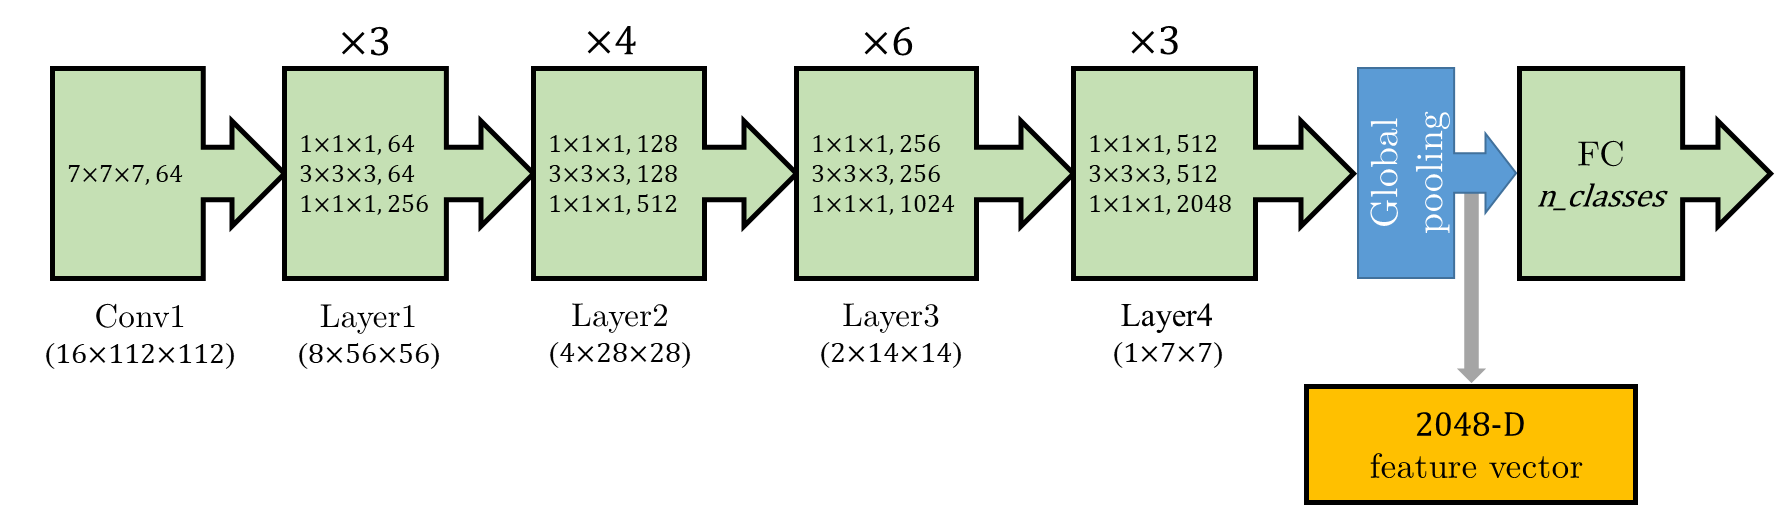
\includegraphics[width=1\linewidth]{Figs/Resnet50_3D.png}
        \caption{Architecture of ResNet-50 3D utilized in our work for feature extraction}
        %\vspace{-0.3cm}
        \label{fig:resnet50_3d}
    \end{figure}

    \textbf{C3D}: 3D deep convolution neural network, which was introduced in \cite{tran2015learning} and has been shown to be very efficient for action recognition tasks. C3D takes input as an image sequence instead of a static image, computes the 3D convolution on each 3D cubes from video clip. By doing so, C3D captures both spatial and temporal characteristics of action at the same time.
    \begin{figure}[htbp]
        \centering
        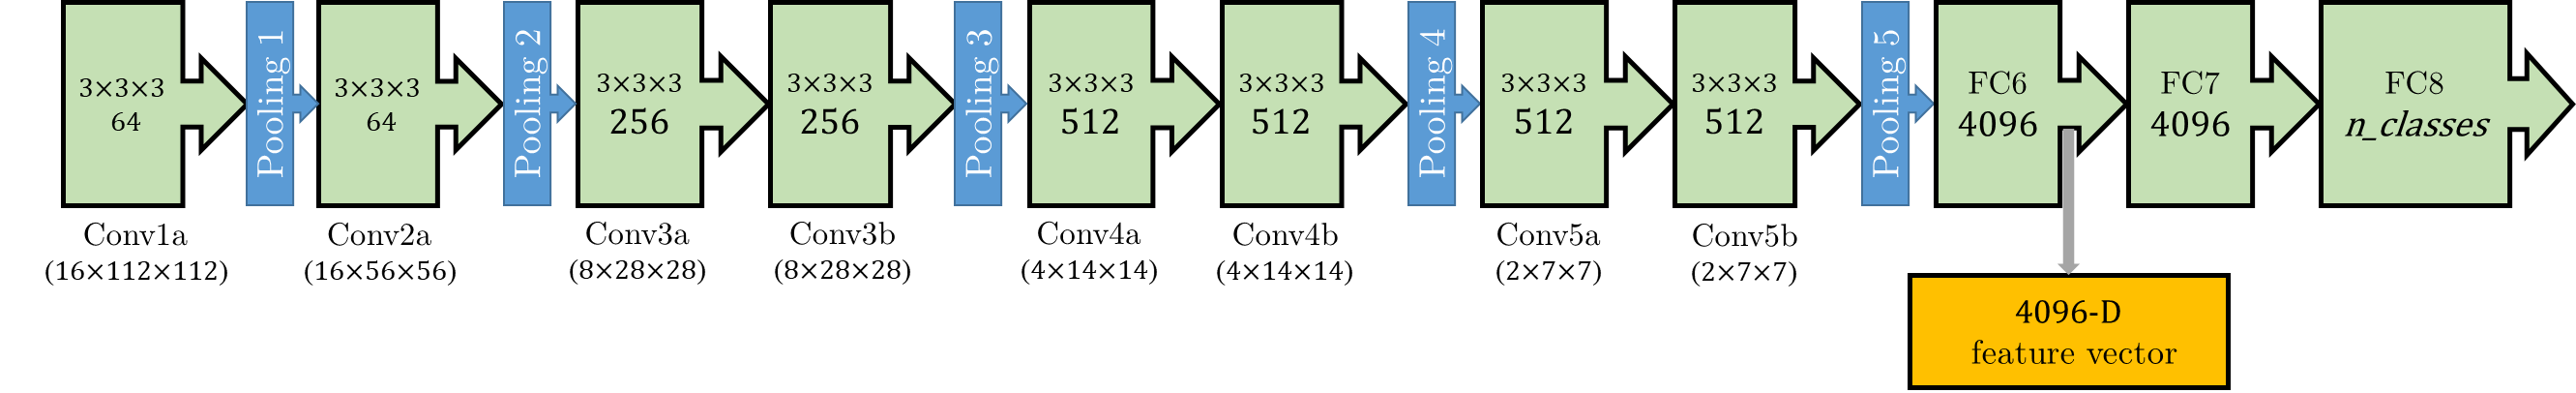
\includegraphics[width=1\linewidth]{Figs/C3D.png}
        \caption{Architecture of C3D utilized in our work for feature extraction}
        %\vspace{-0.3cm}
        \label{fig:C3D}
    \end{figure}
    A C3D network contains 8 convolution, 5 max-pooling and 2 fully connected layers as illustrated in Fig. \ref{fig:C3D}. 
    % The number of filters of convolution layers from Conv1 to Conv5 are 64, 128, 256, 512, 512 respectively. All 3D convolution kernels are of size $3\times3\times3$ with stride $1\times1\times1$ and followed by a 3D batch normalization layer. 
    We utilize the network pre-trained on Sports-1M and fine-tuned on Kinetics dataset.
    To apply in our framework of hand gestures, we apply transfer learning technique on each data stream.
    The feature vector of 4096 dimensions extracted from FC\-6 layer will be served for training and testing classifiers in further steps.
    Details of training the networks as feature extractor for individual views will be presented in Chapter \ref{chap:experimental_result}.
